\section{Дифракционная решетка. Амплитудные и фазовые дифракционные решетки. Дифракционная решетка как спектральный прибор. Разрешающая способность дифракционной решетки. Критерий Рэлея}

\subsection{Дифракционная решетка}

\Def{Дифракционная решетка} --- спектральный прибор,предназначенный для разложения света в спектр и измерения длин волн. Ширину щели как правило обозначают $a$, ширину непрозрачной части экрана между щелями --- $b$. Величина $d = a + b$ --- период решетки. Дифракционная картина наблюдается по методу Фраунгофера.

\begin{figure}[H]
	\centering
	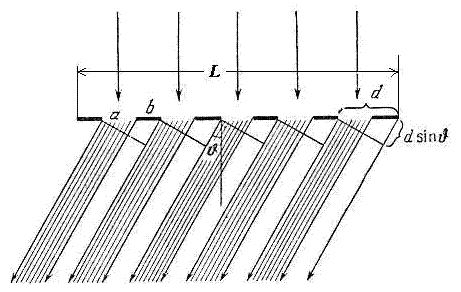
\includegraphics{33_1}
\end{figure}

Здесь угол $\upsilon$ --- угол дифракции.

Разность хода между вторичными волнами, исходящими из соседних щелей $d\sin{\upsilon}$, а разность фаз $\delta = k d\sin{\upsilon}=\frac{2\pi}{\lambda}d\sin{\upsilon}$

Если $E_i$ -- вклад в поле, измеренное в точке наблюдения от $i$-той щели, то:

\begin{align*}
	E_1 &= a\frac{\sin{\alpha}}{\alpha}, \alpha = \frac{kb\sin{\upsilon}}{\upsilon}\\
	E_2 &= E_1 e^{(-i\delta)}\\
	E_3 &= E_1 e^{(-2i\delta)}, E_N = E_1 e^{(-(N-1)i\delta)}
\end{align*}

Для N щелей поле представляется суммой:

\begin{equation*}
	E = E_1[1+e^{(-i\delta)} + ... + e^{(-(N-1)i\delta)}] = E_1\frac{1-e^{(-Ni\delta)}}{1-e^{(-i\delta)}} = E_1\frac{\sin{N\delta/2}}{\sin{\delta/2}}e^{-i(N-1)\delta/2}
\end{equation*}

Тогда интенсивность выражается через интенсивность одной щели:

\begin{equation*}
	I = I_1[\frac{\sin{N\delta/2}}{\sin{\delta/2}}]^2
\end{equation*}

Для особых случаев $\upsilon=0$ и $d\sin{\upsilon}=m\lambda$ формулы дают следующие результаты:

\begin{equation*}
	A=A_1 N, I = I_1 N^2
\end{equation*}

В направлениях, определяемых этим условием,получаются главные максимумы. Интенсивность в соответствующих точках превышает исходную в $N^2$ раз. 

\Def{Условие главных максимумов}: $d\sin{\upsilon}=m\lambda$

Здесь целое число $m$ --- порядок спектра.

Однако при некоторых значениях m максимум может не возникнуть, например, если он максимум одной щели накладывается на минимум другой. При a = b каждый второй максимум не будет виден и условие главных максимумом будет совпадать с условием дифракционного минимума одной щели: $d = a+b = 2a, 2a \sin{\upsilon} = 2n \lambda$

\Def{Условие дифракционного минимума одной щели}: $a \sin{\upsilon} = (m + 1/2) \lambda$ 

Для поиска дифракционных минимумов посмотрим, при каком условии формула интенсивности зануляется:

\begin{equation*}
 \begin{cases}
   \sin\left(\dfrac{N \delta}{2}\right) = 0 \\
	\sin\left(\dfrac{\delta}{2}\right) \ne 0
 \end{cases}
\end{equation*}

\begin{equation*}
	N\delta/2=(Nm+p)\pi, \qlrq d\sin{\upsilon}=(m+\frac{p}{N})\lambda, p = 1, 2, ..., N-1
\end{equation*}

Между двумя соседними минимума будут возникать второстепенные максимумы. Между двумя главными максимумами располагаются $N-1$ минимумов и $N-2$ второстепенных максимумов.

Найти величину $\delta$ можно найти по приближенной формуле:

\begin{equation*}
	N\delta/2=\frac{(Nm+p)\pi}{2}+\frac{(N(m+1)+p)\pi}{2} \qlrq \delta/2=(m+\frac{2p+1}{2N})\pi
\end{equation*}

Дифракционная картина выглядит следующим образом:

\begin{figure}[H]
	\centering
	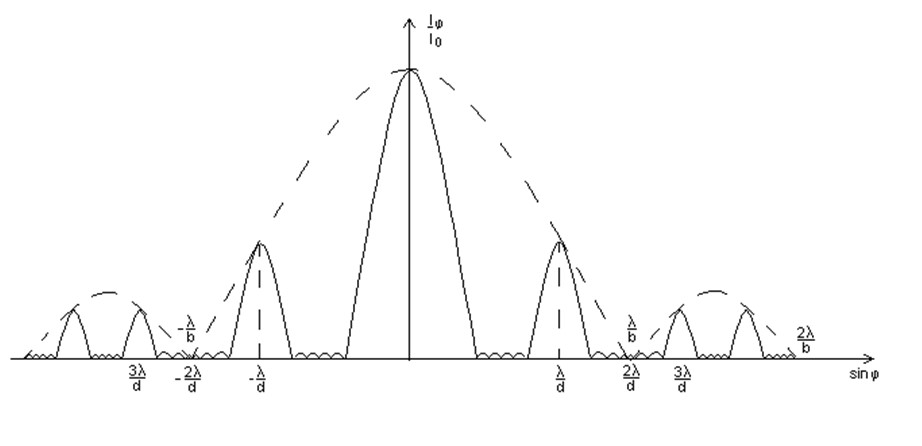
\includegraphics[width=\textwidth]{33_2}
\end{figure}

Если волна падает под углом, разность хода между соседними пучками $d(\sin{\upsilon} - \sin{\upsilon_0})$. Характер дифракционной картины сохранится, но условия минимумов и максимумов изменятся:

\begin{itemize}
	\item \textbf{Условие главных максимумов}:
	
	\begin{equation*}
		d(\sin{\upsilon}-\sin{\upsilon_0})=m\lambda
	\end{equation*}
	
	\item \textbf{Условие дифракционного минимума одной щели}:
	
	\begin{equation*}
		d(\sin{\upsilon}-\sin{\upsilon_0})=(m+p/N)\lambda
	\end{equation*}
\end{itemize}

Дифракционную решетку используют для измерения длины волны.

\subsection{Амплитудные и фазовые дифракционные решетки}

\Def{Амплитудная решетка} Решетка, вносящая периодические изменения в амплитуду волны, не влияя на ее фазу.
Примером является рассмотренная выше решетка.

\Def{Фазовая решетка} Решетка, вносящая  периодические изменения в фазу волны, не влияя на ее амплитуду.

\begin{figure}[H]
	\centering
	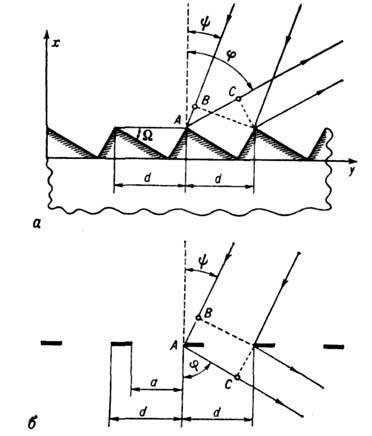
\includegraphics[scale=0.5]{33_3}
	\caption{а) Фазовая решетка; б) Амплитудная решетка}
\end{figure} 

\subsection{Дифракционная решетка как спектральный прибор}
Положение главных максимумов ненулевого порядка зависит от длины волны, значит, всякий сложный свет при прохождении через дифракционную решетку будет раскладываться в спектр:  отдельные монохроматические компоненты разделятся, отклонившись на разные углы. Дифракционные максимумы 1 порядка образуют спектр 1 порядка, затем образуется спектр 2, 3 порядка и т.д.

Спектр называется нормальным, если координата x, характеризующая положение спектральной линии, меняется линейно с длиной волны. Решетка дает нормальный спектр на малых углах.

\begin{figure}[H]
	\centering
	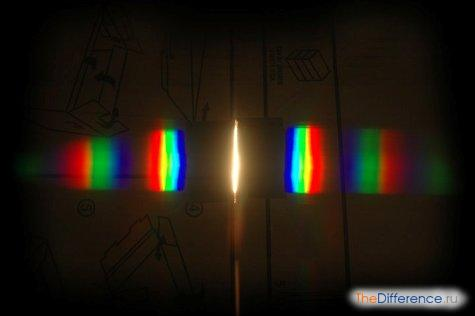
\includegraphics[scale=0.5]{33_4}
\end{figure} 

\subsection{Разрешающая способность дифракционной решетки}

\Def{Угловая дисперсия}: производная $\dfrac{d\upsilon}{d\lambda}=\dfrac{m}{d\cos{\upsilon}}=\dfrac{\sin{\upsilon}-\sin{\upsilon_0}}{\lambda\cos{\upsilon}}$. Не зависит от параметров решетки.

\Def{Дисперсионная область} Максимальная ширина спектрального интервала $\Delta\lambda$, при которой еще нет перекрытия спектров соседних порядков. Крайний случай --- правый конец спектра $m+1$ порядка для длины волны $\lambda$совпадает с левым концом спектра порядка $m$ для длины волны $\lambda'$. Тогда:

\begin{align*}
	d(\sin{\upsilon}-\sin{\upsilon_0})=m\lambda'=(m+1)\lambda\\
	\lambda'-\lambda=\Delta\lambda=\frac{\lambda}{m}
\end{align*} 

Большая дисперсия еще не говорит о том, что две спектральные линии воспринимаются при наблюдении как раздельные объекты,так как любой спектральный аппарат изображает линию как размытую полосу с собственными максимумами и минимумами(дисперсия).Чем более узкие спектральные линии, тем на меньшее расстояние надо их развести, чтобы "разрешить" их. Широкие и сильно размытые линии дадут дифракционную картину одной спектральной линии.
 
\Def{разрешающая способность аппарата}: величина $R=\dfrac{\lambda}{\delta\lambda}$ называется разрешающей способностью аппарата, где $\delta\lambda$ --- наименьшая разность длин волн двух спектральных линий, при которой спектральный аппарат разрешает их.

\subsection{Критерий Рэлея}

Критерий спектрального разрешение дифракционной решетки. Спектральные линии с близкими длинами волн называются разрешенными, если главный максимум дифракционной картины совпадает с первым дифракционным минимумом в том же порядке для другой длины волны. 

\begin{align*}
	d(\sin{\upsilon}-\sin{\upsilon_0})=m\lambda'=(m+\frac{1}{N})\lambda\\
	\delta\lambda=\frac{\lambda}{Nm} \qrq R=Nm
\end{align*}

\begin{figure}[H]
	\centering
	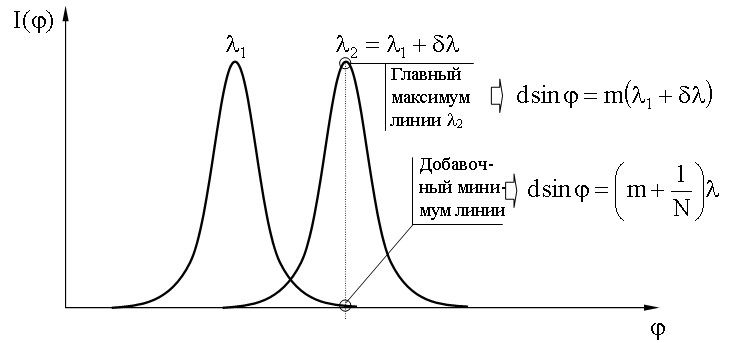
\includegraphics[width=\textwidth]{33_5}
\end{figure} 

Такого вида картина интенсивности позволяет явно увидеть 2 полосы вместо 1.
